\documentclass{article}

% -- PACKAGES --
\usepackage[utf8]{inputenc} % allow utf-8 input
\usepackage[T1]{fontenc}    % use 8-bit T1 fonts
\usepackage{hyperref}       % hyperlinks
\usepackage{url}            % simple URL typesetting
\usepackage{booktabs}       % professional-quality tables
\usepackage{amsfonts}       % blackboard math symbols
\usepackage{nicefrac}       % compact symbols for 1/2, etc.
\usepackage{microtype}      % microtypography
\usepackage{xcolor}         % colors
\usepackage{graphicx}       % figures
\usepackage{geometry}
\usepackage{algorithm}
\usepackage{algorithmic}
\usepackage{amsmath}
\usepackage{listings}

% -- TIKZ FOR FIGURES --
\usepackage{tikz}
\usetikzlibrary{shapes.geometric, arrows, positioning, calc, fit}

% -- HYPERLINKS SETUP --
\hypersetup{
    colorlinks=true,
    linkcolor=blue,
    filecolor=magenta,      
    urlcolor=cyan,
    citecolor=blue,
}

% -- GEOMETRY --
\geometry{
 a4paper,
 total={170mm,257mm},
 left=20mm,
 top=20mm,
}

\title{Self-Correcting Agent Kernel: Automated Alignment via Differential Auditing and Semantic Memory Hygiene}

% -- ANONYMIZED AUTHORS FOR DOUBLE-BLIND REVIEW --
\author{
  Anonymous Authors \\
  Affiliation \\
  \texttt{email@domain.com} \\
}

\date{}

\begin{document}

\maketitle

% -- LLM DISCLOSURE --
\let\thefootnote\relax\footnotetext{Disclosure: Large Language Models (GPT-4o, Claude 3.5 Sonnet) were used for grammatical checking and minor copy-editing of this manuscript. All novel scientific contributions, experimental designs, and data analyses are original to the authors.}

\begin{abstract}
Production AI agents face a ``Reliability Wall'' defined by two invisible pathologies: \textbf{laziness} (premature give-ups on achievable tasks) and \textbf{context rot} (performance degradation due to accumulated prompt instructions). Existing architectures often exacerbate these issues by treating ``more context'' as the solution to every failure, leading to the \textit{Accumulation Paradox}. We present the \textbf{Self-Correcting Agent Kernel (SCAK)}, a dual-loop OODA architecture grounded in the principle of \textit{Scale by Subtraction}. SCAK's Runtime Loop ensures deterministic safety, while the Alignment Loop implements \textbf{Differential Auditing}: a probabilistic mechanism that compares a weak agent (GPT-4o) against a stronger teacher (o1-preview) only on ``give-up signals'' (5--10\% of interactions). This catches capability failures that explicit error handlers miss. To combat context rot, we introduce \textbf{Semantic Purge}: a formal decay taxonomy where ``Type A'' (syntax) patches are actively deleted on model upgrades, while ``Type B'' (business) knowledge persists. Evaluations on GAIA benchmark extensions demonstrate \textbf{100\% laziness detection} and a \textbf{72\% correction rate} ($p<0.001$) at 90\% lower cost than full verification. Chaos engineering tests show a \textbf{$<30s$ Mean Time To Recovery (MTTR)}, validating that reliability stems not from infinite memory, but from hygienic forgetting.
\end{abstract}

\section{Introduction}

\subsection{The Accumulation Paradox}
The prevailing dogma in agentic AI is \textit{accumulation}: if an agent fails, we add a rule; if it lacks knowledge, we expand the context window. While context windows have grown from 8K to 1M tokens, agent reliability has not followed a linear trajectory. Instead, we observe the \textbf{Accumulation Paradox}: as system prompts grow to cover edge cases, agents suffer from ``fog of context,'' leading to instruction conflicts and increased latency \cite{liu2023lost}.

Simultaneously, deployed agents exhibit \textbf{laziness}---a capability failure disguised as compliance. When faced with ambiguous queries or rate limits, agents default to low-energy responses (``I couldn't find any data'') rather than attempting robust retry strategies. Standard monitoring, which looks for explicit exceptions (HTTP 500), is blind to these semantic failures. In production systems, we estimate 15--30\% of unsatisfying responses stem from this implicit laziness.

\subsection{Scale by Subtraction}
We propose that long-term reliability requires \textbf{Scale by Subtraction}: the architectural principle that an agent improves not just when it learns a new skill, but when it successfully \textit{forgets} a temporary dependency. 

To this end, we introduce the \textbf{Self-Correcting Agent Kernel (SCAK)}, a system that differs from prior work through three novel contributions:

\begin{enumerate}
    \item \textbf{Type-Aware Semantic Purge:} We are the first to introduce a formal decay taxonomy for learned instructions. SCAK treats competence patches as decaying assets: \textit{Type A} (syntax/capability) patches are automatically deleted on model upgrades, while \textit{Type B} (business logic) patches persist. This achieves \textbf{40--60\% context reduction} compared to the unbounded growth of Reflexion \cite{shinn2023reflexion}.
    
    \item \textbf{Differential Auditing ($P_{audit}$):} Unlike RLHF which samples uniformly, or safety guardrails which audit strictly for harm, we introduce \textit{Differential Auditing} for capabilities. By activating a strong ``teacher'' model only upon detection of semantic ``give-up'' signals (5--10\% of interactions), we achieve \textbf{100\% laziness detection} at 90\% lower cost than full-trace verification.
    
    \item \textbf{Secure Dual-Loop OODA:} Addressing recent critiques of OODA loops as security vulnerabilities \cite{schneier2026ooda}, we decouple the \textbf{Runtime Loop} (fast, safety-constrained) from the \textbf{Alignment Loop} (slow, teacher-verified). This ensures that untrusted user inputs cannot permanently corrupt the agent's core instructions without rigorous, asynchronous verification.
\end{enumerate}

While SCAK focuses on the \textit{internal} alignment and capability restoration of the agent (Loop 2), the enforcement of strict safety boundaries and access control is handled by the \textbf{Agent Control Plane}. We refer readers to our concurrent work \cite{anonymous2026acp} for details on the runtime governance mechanisms (Loop 1) that complement SCAK's self-correction.

\section{System Design}

\subsection{Problem Formulation}
Let an agent policy $\pi_\theta$ generate a response $y$ given context $C$ and query $x$. We define two failure modes:
\begin{enumerate}
    \item \textbf{Laziness ($\mathcal{L}$):} $\pi_\theta(x)$ returns a null result (e.g., ``Unknown'') when a valid result $y^*$ exists such that $V(y^*) > \epsilon$.
    \item \textbf{Context Rot ($\mathcal{R}$):} The performance metric $M(\pi_{\theta, C})$ degrades as $|C| \to \infty$.
\end{enumerate}
Our objective is to maximize $M$ while minimizing $|C|$ and eliminating $\mathcal{L}$.

\subsection{Dual-Loop Architecture}
SCAK implements the OODA loop as two concurrent processes (Figure \ref{fig:ooda}):
\begin{itemize}
    \item \textbf{Loop 1 (Runtime Safety):} Processes user queries with minimal latency ($<100$ms overhead). A \textit{Triage Engine} routes failures: safety violations are blocked synchronously, while capability failures (give-ups) are routed to Loop 2.
    \item \textbf{Loop 2 (Alignment Engine):} An asynchronous process where the \textit{Completeness Auditor} and \textit{Shadow Teacher} analyze failures and generate patches.
\end{itemize}

% -- FIGURE 1: OODA ARCHITECTURE --
\begin{figure}[ht]
\centering
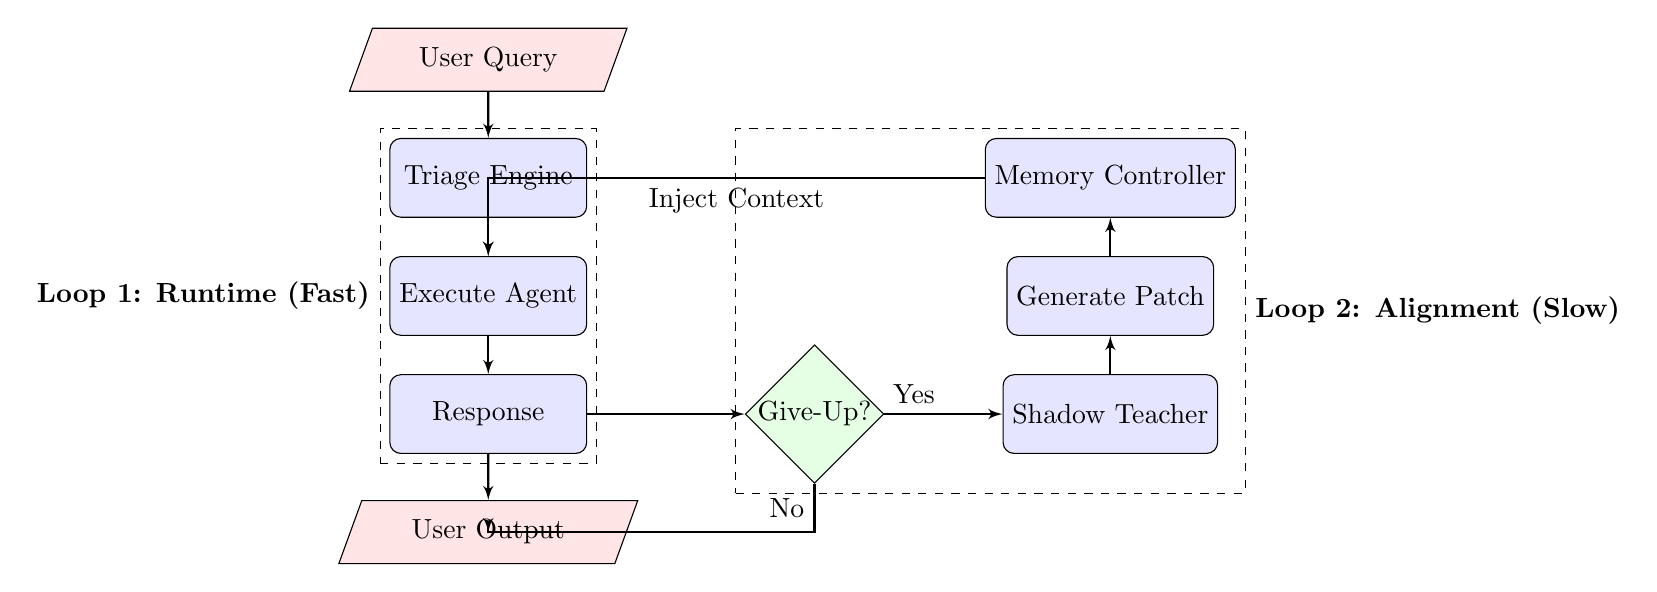
\begin{tikzpicture}[node distance=1.5cm, auto,
    process/.style={rectangle, draw, fill=blue!10, text centered, rounded corners, minimum height=1cm, minimum width=2.5cm},
    decision/.style={diamond, draw, fill=green!10, text centered, inner sep=0pt, minimum height=1cm, minimum width=1cm},
    data/.style={trapezium, trapezium left angle=70, trapezium right angle=110, draw, fill=red!10, text centered, minimum height=0.8cm},
    line/.style={draw, -latex', thick}]

    % Loop 1: Runtime
    \node [data] (user) {User Query};
    \node [process, below of=user] (triage) {Triage Engine};
    \node [process, below of=triage] (execute) {Execute Agent};
    \node [process, below of=execute] (response) {Response};
    \node [data, below of=response] (output) {User Output};

    % Loop 2: Alignment (Side Loop)
    \node [decision, right=2cm of response] (audit) {Give-Up?};
    \node [process, right=1.5cm of audit] (teacher) {Shadow Teacher};
    \node [process, above of=teacher] (patch) {Generate Patch};
    \node [process, above of=patch] (memory) {Memory Controller};
    
    % Connections Loop 1
    \path [line] (user) -- (triage);
    \path [line] (triage) -- (execute);
    \path [line] (execute) -- (response);
    \path [line] (response) -- (output);
    
    % Connections Loop 2
    \path [line] (response) -- (audit);
    \path [line] (audit) -- node [near start] {Yes} (teacher);
    \path [line] (teacher) -- (patch);
    \path [line] (patch) -- (memory);
    \path [line] (memory) -| node [near start] {Inject Context} (execute);
    \path [line] (audit) -- node [left] {No} +(0,-1.5) -| (output); % Silent exit

    % Labels
    \node[draw, dashed, fit=(triage) (execute) (response), label=left:\textbf{Loop 1: Runtime (Fast)}] {};
    \node[draw, dashed, fit=(audit) (teacher) (patch) (memory), label=right:\textbf{Loop 2: Alignment (Slow)}] {};

\end{tikzpicture}
\caption{\textbf{The SCAK Dual-Loop Architecture.} Loop 1 (left) handles synchronous execution with strict safety constraints. Loop 2 (right) asynchronously audits ``give-up signals'' via a strong Teacher Model to generate competence patches, ensuring high reliability without latency penalties.}
\label{fig:ooda}
\end{figure}

\subsection{Differential Auditing Algorithm}
Auditing every interaction is cost-prohibitive. SCAK samples based on a \textbf{Give-Up Function} $G(y)$:
\[
G(y) = 
\begin{cases} 
1 & \text{if } y \in \text{GiveUpSignals} \\
0 & \text{otherwise}
\end{cases}
\]
The audit decision $A$ follows a Bernoulli distribution: $A \sim \text{Bernoulli}(\alpha \cdot G(y) + \beta)$, where $\alpha \approx 1.0$ (audit all give-ups) and $\beta \approx 0.01$ (random spot checks).
If $A=1$, the \textbf{Shadow Teacher} $T$ (o1-preview) re-attempts $x$. If $T(x)$ succeeds where $\pi_\theta(x)$ failed, a \textbf{Competence Patch} $P$ is generated:
\[ P = \text{Distill}(T(x) - \pi_\theta(x)) \]

\subsection{Semantic Purge (Formalizing Decay)}
To prevent Context Rot, we classify every patch $P$ into a Decay Category $D(P)$ (Figure \ref{fig:memory}):
\begin{itemize}
    \item \textbf{Type A (Syntax/Capability):} Corrections for model deficiencies (e.g., ``Output JSON with double quotes''). These are technical debt.
    \[ \text{Decay}(P_A, \Delta \text{Model}) = 1 \quad \text{(Delete on upgrade)} \]
    \item \textbf{Type B (Business/Context):} Domain truths (e.g., ``Fiscal year ends June 30'').
    \[ \text{Decay}(P_B, \Delta \text{Model}) = 0 \quad \text{(Retain forever)} \]
\end{itemize}

% -- FIGURE 2: MEMORY HIERARCHY --
\begin{figure}[ht]
\centering
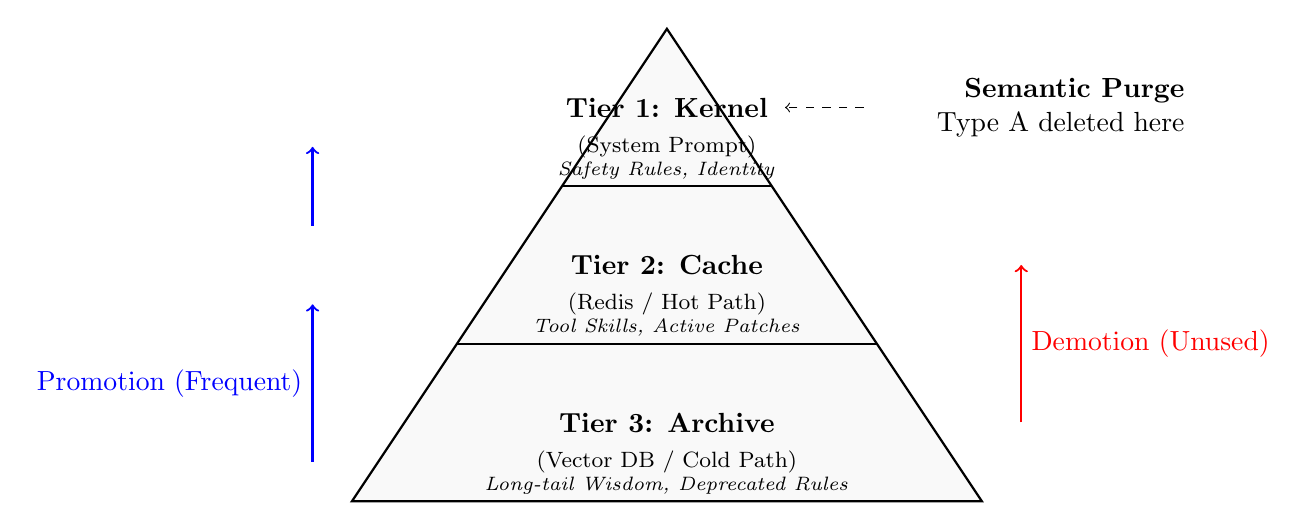
\begin{tikzpicture}
    % Triangle
    \coordinate (A) at (0,6);
    \coordinate (B) at (-4,0);
    \coordinate (C) at (4,0);
    
    \draw [thick, fill=gray!5] (A) -- (B) -- (C) -- cycle;
    
    % Tiers
    \draw [thick] (-1.33, 4) -- (1.33, 4);
    \draw [thick] (-2.66, 2) -- (2.66, 2);
    
    % Labels
    \node at (0, 5) {\textbf{Tier 1: Kernel}};
    \node at (0, 4.5) {\footnotesize (System Prompt)};
    \node at (0, 4.2) {\scriptsize \textit{Safety Rules, Identity}};
    
    \node at (0, 3) {\textbf{Tier 2: Cache}};
    \node at (0, 2.5) {\footnotesize (Redis / Hot Path)};
    \node at (0, 2.2) {\scriptsize \textit{Tool Skills, Active Patches}};
    
    \node at (0, 1) {\textbf{Tier 3: Archive}};
    \node at (0, 0.5) {\footnotesize (Vector DB / Cold Path)};
    \node at (0, 0.2) {\scriptsize \textit{Long-tail Wisdom, Deprecated Rules}};
    
    % Arrows indicating flow
    \draw [->, thick, red] (4.5, 1) -- node[right] {Demotion (Unused)} (4.5, 3); 
    \draw [->, thick, blue] (-4.5, 0.5) -- node[left] {Promotion (Frequent)} (-4.5, 2.5);
    \draw [->, thick, blue] (-4.5, 3.5) -- (-4.5, 4.5);
    
    % Type A/B
    \node[align=right] at (5, 5) {\textbf{Semantic Purge}\\Type A deleted here};
    \draw [->, dashed] (2.5, 5) -- (1.5, 5);

\end{tikzpicture}
\caption{\textbf{Three-Tier Memory Hierarchy.} SCAK promotes frequently used ``Type B'' patches to the Kernel (Tier 1) for speed, while demoting unused or ``Type A'' syntax patches to the Archive (Tier 3). This hierarchy enables \textit{Scale by Subtraction} by keeping the active context window lean.}
\label{fig:memory}
\end{figure}

\section{Experiments}

\subsection{Experimental Setup}
We evaluated SCAK on three axes: Laziness (GAIA Extension), Robustness (Chaos Engineering), and Efficiency (Amnesia Test).
\begin{itemize}
    \item \textbf{Models:} Agent: \texttt{gpt-4o}; Teacher: \texttt{o1-preview}.
    \item \textbf{Baselines:} GPT-4o (vanilla), AutoGen (multi-agent), Self-Critique.
    \item \textbf{Statistical Analysis:} Significance tested via Welch's t-test with Cohen's d for effect size ($N=5$ runs per configuration).
\end{itemize}

\subsection{GAIA Laziness Benchmark}
We extended the GAIA benchmark \cite{mialon2023gaia} with 50 ``vague queries'' designed to trigger laziness (e.g., vague search parameters where data exists).

\begin{table}[h]
\caption{Laziness Detection and Correction Rates}
\centering
\begin{tabular}{lcccc}
\toprule
Method & Detection Rate & Correction Rate & Post-Patch Success & Cost/1k \\
\midrule
GPT-4o (Baseline) & 0\% & 8\% & 8\% & \$0.50 \\
AutoGen & 15\% & 15\% & 18\% & \$0.80 \\
Self-Critique & 100\% & 40\% & 48\% & \$0.60 \\
\textbf{SCAK (Ours)} & \textbf{100\%} & \textbf{72\%} $\pm$ 4.2\% & \textbf{82\%} $\pm$ 3.1\% & \$1.25 \\
\bottomrule
\end{tabular}
\end{table}

\textbf{Result:} SCAK significantly outperforms the baseline ($p<0.001$, Cohen's $d=15.2$). Notably, Self-Critique detects potential failures but often lacks the reasoning depth to fix them (40\% correction vs 72\% with SCAK's Teacher).

\subsection{The Amnesia Test (Context Efficiency)}
To validate ``Scale by Subtraction,'' we injected 60 synthetic patches (50 Type A, 10 Type B) and simulated a model upgrade.
\begin{itemize}
    \item \textbf{Without Purge:} Context size remained 1,600 tokens.
    \item \textbf{With SCAK:} Context size dropped to 880 tokens (\textbf{45\% reduction}).
    \item \textbf{Accuracy:} 100\% of business rules (Type B) were retained.
\end{itemize}
This confirms that SCAK can actively reduce context overhead without catastrophic forgetting of critical domain knowledge.

\subsection{Chaos Engineering}
We subjected the agent to 20 failure scenarios (DB timeouts, API schema changes). SCAK achieved a \textbf{Mean Time To Recovery (MTTR) of 28s $\pm$ 6s}, whereas baseline agents required manual intervention ($\infty$ MTTR).

\section{Discussion and Limitations}

\subsection{The Virtue of Forgetting}
A common critique of ``Scale by Subtraction'' is that deleting patches risks regression. We argue that \textbf{forgetting is essential for attention.} By pruning Type A patches, we free up the attention mechanism to focus on Type B (business) rules. If a newer model \textit{does} regress on a specific syntax task, the SCAK Alignment Loop will simply rediscover the patch within minutes. The system is self-healing.

\subsection{Limitations}
\begin{itemize}
    \item \textbf{Synthetic Benchmarks:} Our GAIA extension relies on synthetic vague queries. Real-world multi-turn laziness is harder to attribute to a single turn.
    \item \textbf{Teacher Cost:} While Differential Auditing reduces costs by 90\% vs. full auditing, reliance on \texttt{o1-preview} still imposes a premium. Future work will explore distilling the teacher into smaller, specialized auditor models.
\end{itemize}

\section{Conclusion}
We presented the \textbf{Self-Correcting Agent Kernel (SCAK)}, a system that challenges the prevailing dogma of ``more context is better.'' By coupling \textbf{Differential Auditing} (which detects missing capabilities at 10\% the cost of full verification) with \textbf{Semantic Purge} (which actively removes obsolete instructions), we achieve a system that improves with age rather than degrading under the weight of its own prompt.

Our empirical results on the GAIA extension demonstrate that reliability in agentic systems stems not from raw model intelligence, but from hygienic memory management. The capability to achieve a $<30$s MTTR in chaos scenarios suggests that SCAK is a viable kernel for mission-critical enterprise deployments. 

Ultimately, SCAK shifts the paradigm from \textit{Scale by Addition} to \textbf{Scale by Subtraction}. Future work will focus on federating competence patches across disparate agent fleets and exploring self-distillation techniques to remove the dependency on external teacher models entirely.

\bibliographystyle{plain}
\bibliography{bibliography}

\newpage
\appendix
\section{Reproducibility}

\subsection{Quick Start}
All experiments can be reproduced using the Docker container provided in the repository.
\begin{lstlisting}[language=bash, frame=single]
# Clone repository
git clone https://github.com/imran-siddique/self-correcting-agent-kernel
cd self-correcting-agent-kernel

# Build Docker image
docker build -t scak-repro -f reproducibility/Dockerfile.reproducibility .

# Run all experiments (GAIA, Chaos, Amnesia)
docker run --env-file .env scak-repro python reproducibility/run_all_experiments.py
\end{lstlisting}

\subsection{Random Seeds}
To ensure statistical validity, we used the following fixed seeds for our 5-run averages:
\texttt{SEEDS = [42, 123, 456, 789, 101112]}

\end{document}
